%%%%%%%%%%%%%%%%%%%%%%%%%%%%%%%%%%%%%%%%%%%%%%%%%%%%%%%%%%%%%%%%%%%%%%
% Overleaf (WriteLaTeX) Example: Molecular Chemistry Presentation
%
% Source: http://www.overleaf.com
%
% In these slides we show how Overleaf can be used with standard 
% chemistry packages to easily create professional presentations.
% 
% Feel free to distribute this example, but please keep the referral
% to overleaf.com
% 
%%%%%%%%%%%%%%%%%%%%%%%%%%%%%%%%%%%%%%%%%%%%%%%%%%%%%%%%%%%%%%%%%%%%%%

\documentclass{beamer}

\mode<presentation>
{
  \usetheme{Madrid}       % or try default, Darmstadt, Warsaw, ...
  \usecolortheme{default} % or try albatross, beaver, crane, ...
  \usefonttheme{default}    % or try default, structurebold, ...
  \setbeamertemplate{navigation symbols}{}
  \setbeamertemplate{caption}[numbered]
} 

\usepackage[english]{babel}
\usepackage[utf8x]{inputenc}
\usepackage{graphicx}
\usepackage{hyperref}
  \hypersetup{colorlinks=true}
  \hypersetup{urlcolor=blue}
  \hypersetup{linkcolor = .}
\usepackage{xcolor}
\usepackage{siunitx}
  \sisetup{separate-uncertainty = true}
\usepackage{physics}
\usepackage[font=small,labelfont=bf]{caption}
\usepackage{subcaption}
\usepackage[en-GB]{datetime2}
\usepackage{overpic}
\usepackage{feynmp}
\DeclareGraphicsRule{*}{mps}{*}{}
\usepackage{scalerel}
\newcommand{\mylbrace}[2]{\vspace{#2pt}\hspace{6pt}\scaleleftright[\dimexpr5pt+#1\dimexpr0.06pt]{\lbrace}{\rule[\dimexpr2pt-#1\dimexpr0.5pt]{-4pt}{#1pt}}{.}}
\newcommand{\myrbrace}[2]{\vspace{#2pt}\scaleleftright[\dimexpr5pt+#1\dimexpr0.06pt]{.}{\rule[\dimexpr2pt-#1\dimexpr0.5pt]{-4pt}{#1pt}}{\rbrace}\hspace{6pt}}

% Here's where the presentation starts, with the info for the title slide
\title[$K^+K^-\pi^+\pi^-$]{Update on \texorpdfstring{$B^\pm\to Dh^\pm$}{B to Dh}, \texorpdfstring{$D\to K^+K^-\pi^+\pi^-$}{K+K-pi+pi-} analysis at LHCb and BESIII}

\author{Martin Tat}
\institute{Oxford LHCb}
\date{10th January 2022}

\titlegraphic{
\includegraphics[height = 2cm]{lhcb.jpg}\hspace{1cm}~%
              
\includegraphics[height = 2cm]{OxfordLogo.pdf}\hspace{1cm}~%
              
\includegraphics[height = 2cm]{bes3.jpg}}

\begin{document}

\begin{frame}
  \titlepage
\end{frame}

% These three lines create an automatically generated table of contents.
\begin{frame}{Outline}
  \tableofcontents
\end{frame}

\section{LHCb}
\subsection{Summary of current LHCb analysis progression}

\begin{frame}{LHCb analysis summary}
  \begin{itemize}
    \setlength\itemsep{0.5em}
    \item{Previous report on $B^\pm\to Dh^\pm$, $D\to K^+K^-\pi^+\pi^-$:}
    \begin{enumerate}
      \setlength\itemsep{0.5em}
      \item{Global mass fit $\implies$ Obtain mass shape}
      \item{Binned CP fit $\implies$ Obtain CP observables}
      \item{Backgrounds: Charmless, $D\to K\pi\pi\pi\pi^0$, $D\to K\pi\pi\pi$, $D\to K(X)l\nu$}
    \end{enumerate}
  \end{itemize}
  \begin{figure}
    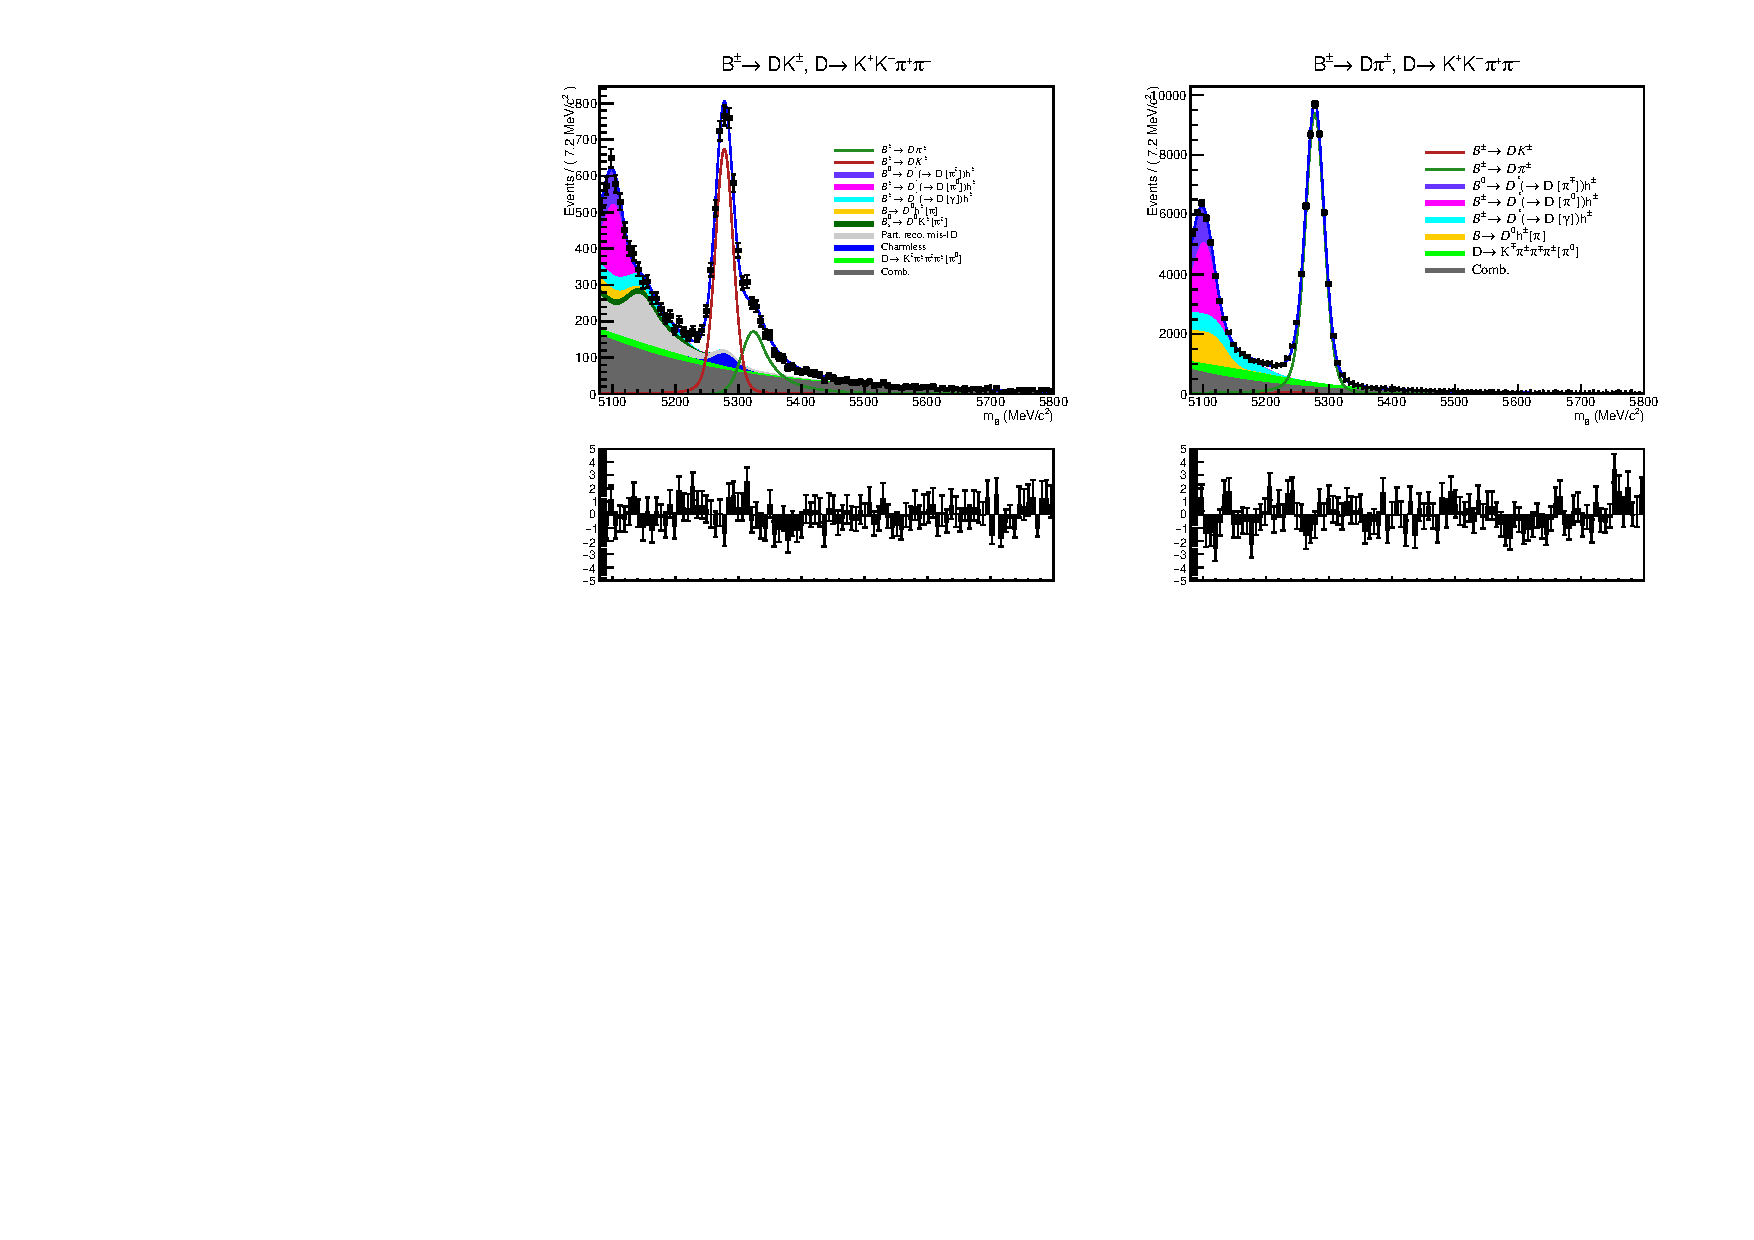
\includegraphics[width = 0.85\textwidth]{Plots/d2kkpipi_fiveL_allDP.pdf}
  \end{figure}
\end{frame}

\begin{frame}{LHCb analysis summary}
  \begin{itemize}
    \setlength\itemsep{0.5em}
    \item{Current analysis progress:}
    \begin{enumerate}
      \setlength\itemsep{0.5em}
      \item{Finished ANA note draft, currently in 1st circulation in B2OC WG}
      \item{Received comments from 2/3 reviewers, replies ready this week}
      \begin{itemize}
        \item{Will request $B\to(K\pi\pi\pi\pi^0)_Dh^\pm$ MC}
        \item{Fit with $c_i$, $s_i$ floated?}
      \end{itemize}
      \item{Need to finish off systematics for:}
      \begin{itemize}
        \item{Charmless and $K\pi\pi\pi\pi^0$ backgrounds}
        \item{$c_i$, $s_i$ model-dependent uncertainties}
      \end{itemize}
    \end{enumerate}
  \end{itemize}
  \begin{figure}
    \centering
    \vspace{-0.2cm}
    \begin{subfigure}{0.30\textwidth}
      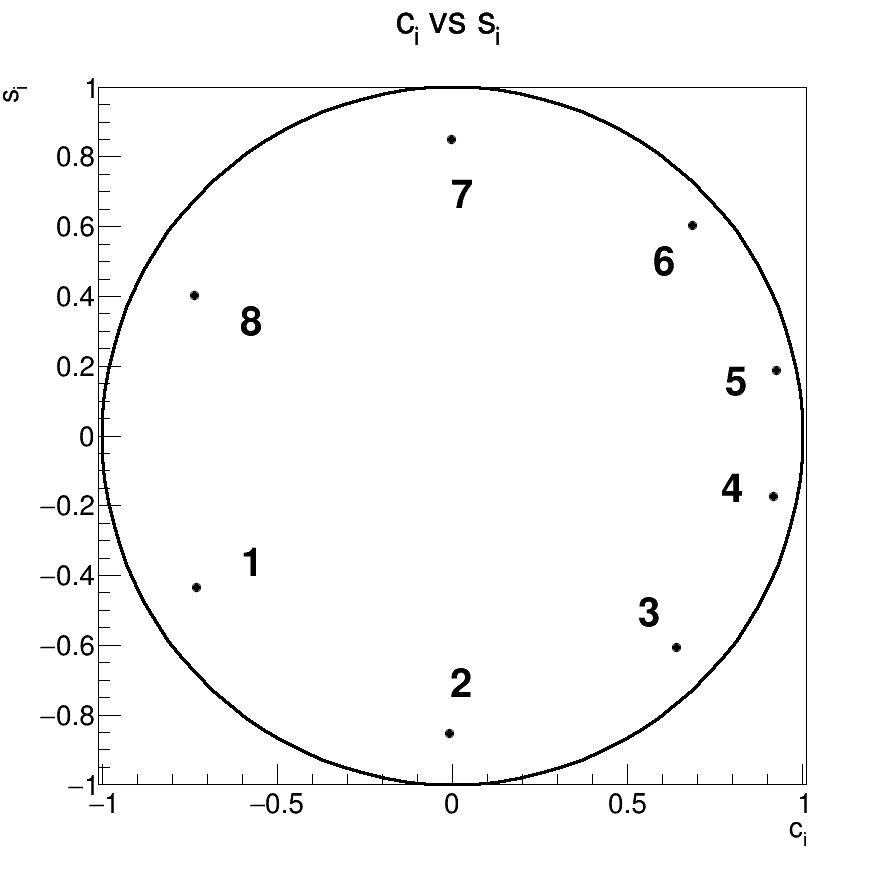
\includegraphics[width = 1.0\textwidth]{Plots/StrongPhaseParametersPlot_cisi_8Bins.png}
      \caption{LHCb model}
    \end{subfigure}%
    \begin{subfigure}{0.30\textwidth}
      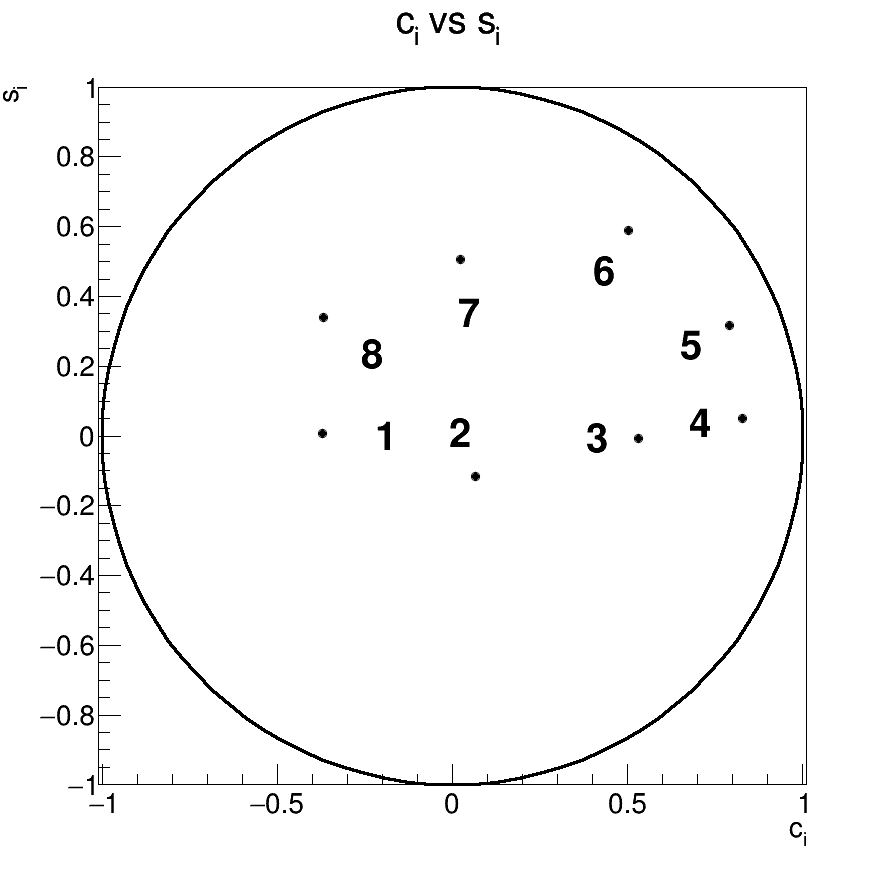
\includegraphics[width = 1.0\textwidth]{Plots/StrongPhaseParametersPlot_Mint2_cisi_8Bins.png}
      \caption{CLEO model}
    \end{subfigure}
  \end{figure}
\end{frame}

\section{BESIII}
\subsection{Strong-phase determination in quantum correlated \texorpdfstring{$D^0\bar{D^0}$}{D0D0} decays}

\begin{frame}{Strong-phase in quantum correlated $D^0\bar{D^0}$ decays}
  \begin{itemize}
    \item{BESIII: $e^+e^-$ collider at $\psi(3770)\to D^0\bar{D^0}$ threshold}
    \begin{itemize}
      \item{2010-2011: $\SI{2.93}{\per\femto\barn}$}
      \item{Since 23rd December: $\SI{0.46}{\per\femto\barn}$}
      \item{Expect $\SI{20}{\per\femto\barn}$ by end of 2023}
    \end{itemize}
  \end{itemize}
  \begin{figure}
    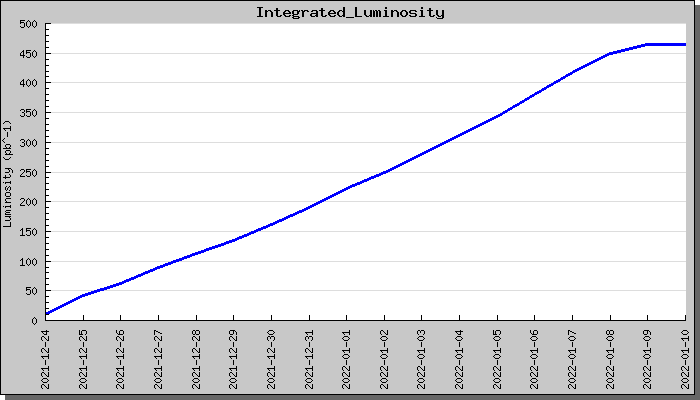
\includegraphics[width = 0.70\textwidth]{Plots/BES3_Integrated_Luminosity.png}
  \end{figure}
\end{frame}

\begin{frame}{Strong-phase in quantum correlated $D^0\bar{D^0}$ decays}
  \begin{itemize}
    \item{Double-tag analysis: Reconstruct signal mode ($KK\pi\pi$) and known tag mode}
    \item{$D^0\bar{D^0}$ pair is quantum correlated}
  \end{itemize}
  \begin{figure}[H]
    \centering
    \vspace{-1.5cm}
    \begin{fmffile}{fgraph/fgraph_ee1}
      \setlength{\unitlength}{1cm}
      \begin{fmfgraph*}(8,5)
        \fmfleft{i}
        \fmfright{o}
        \fmflabel{$D^0$}{i}
        \fmflabel{$\bar{D^0}$}{o}
        \fmf{fermion}{w,i}
        \fmf{fermion}{w,o}
        \fmfblob{1cm}{w}
        \fmfv{label=$\psi(3770)$,label.dist=15,label.angle=90}{w}
      \end{fmfgraph*}
    \end{fmffile}
    \vspace{-1.5cm}
  \end{figure}
  \begin{itemize}
    \item{Equivalently, we can consider $D_+D_-$}
    \begin{itemize}
      \item{$D_\pm = \frac{1}{\sqrt{2}}(D^0\pm\bar{D^0})$ are CP eigenstates}
    \end{itemize}
  \end{itemize}
  \begin{figure}[H]
    \centering
    \vspace{-1.5cm}
    \begin{fmffile}{fgraph/fgraph_ee2}
      \setlength{\unitlength}{1cm}
      \begin{fmfgraph*}(8,5)
        \fmfleft{i}
        \fmfright{o}
        \fmflabel{$D_+$}{i}
        \fmflabel{$D_-$}{o}
        \fmf{fermion}{w,i}
        \fmf{fermion}{w,o}
        \fmfblob{1cm}{w}
        \fmfv{label=$\psi(3770)$,label.dist=15,label.angle=90}{w}
      \end{fmfgraph*}
    \end{fmffile}
    \vspace{-1.5cm}
  \end{figure}
\end{frame}

\begin{frame}{Strong-phase in quantum correlated $D^0\bar{D^0}$ decays}
  \begin{itemize}
    \item{Tag mode can be a \underline{flavour tag}}
    \begin{itemize}
      \item{$K^-\pi^+$, $K^-\pi^+\pi^0$, $K^-\pi^+\pi^-\pi^+$, $K^-e^+\nu_e$}
    \end{itemize}
  \end{itemize}
  \begin{figure}[H]
    \centering
    \vspace{0.3cm}
    \begin{fmffile}{fgraph/fgraph_flavour_tag}
      \setlength{\unitlength}{1cm}
      \begin{fmfgraph*}(8,4)
        \fmfstraight
        \fmfleft{i4,i3,i2,i1}
        \fmfright{g1,o1,o2,g2}
        \fmflabel{$\pi^+$}{o1}
        \fmflabel{$K^-$}{o2}
        \fmflabel{$K^+$}{i1}
        \fmflabel{$K^-$}{i2}
        \fmflabel{$\pi^+$}{i3}
        \fmflabel{$\pi^-$}{i4}
        \fmf{fermion}{w,i1}
        \fmf{fermion}{w,i2}
        \fmf{fermion}{w,i3}
        \fmf{fermion}{w,i4}
        \fmf{fermion}{w,o1}
        \fmf{fermion}{w,o2}
        \fmf{phantom}{w,g1}
        \fmf{phantom}{w,g2}
        \fmfblob{1cm}{w}
      \end{fmfgraph*}
    \end{fmffile}
    \vspace{0.0cm}
  \end{figure}
\end{frame}

\begin{frame}{Strong-phases in quantum correlated $D^0\bar{D^0}$ decays}
  \begin{itemize}
    \item{Tag mode can be a \underline{CP even tag}}
    \begin{itemize}
      \item{$KK$, $\pi\pi$, $\pi\pi\pi^0$, $K_S\pi^0\pi^0$, $K_L\pi^0$, $K_L\omega$}
    \end{itemize}
  \end{itemize}
  \begin{figure}[H]
    \centering
    \vspace{0.3cm}
    \begin{fmffile}{fgraph/fgraph_CPeven_tag}
      \setlength{\unitlength}{1cm}
      \begin{fmfgraph*}(8,4)
        \fmfstraight
        \fmfleft{i4,i3,i2,i1}
        \fmfright{g1,o1,o2,g2}
        \fmflabel{$K^+$}{o1}
        \fmflabel{$K^-$}{o2}
        \fmflabel{$K^+$}{i1}
        \fmflabel{$K^-$}{i2}
        \fmflabel{$\pi^+$}{i3}
        \fmflabel{$\pi^-$}{i4}
        \fmf{fermion}{w,i1}
        \fmf{fermion}{w,i2}
        \fmf{fermion}{w,i3}
        \fmf{fermion}{w,i4}
        \fmf{fermion}{w,o1}
        \fmf{fermion}{w,o2}
        \fmf{phantom}{w,g1}
        \fmf{phantom}{w,g2}
        \fmfblob{1cm}{w}
      \end{fmfgraph*}
    \end{fmffile}
    \vspace{0.0cm}
  \end{figure}
\end{frame}

\begin{frame}{Strong-phase in quantum correlated $D^0\bar{D^0}$ decays}
  \begin{itemize}
    \item{Tag mode can be a \underline{CP odd tag}}
    \begin{itemize}
      \item{$K_S\pi^0$, $K_S\omega$, $K_S\eta$, $K_S\eta'$, $K_L\pi^0\pi^0$}
    \end{itemize}
  \end{itemize}
  \begin{figure}[H]
    \centering
    \vspace{0.3cm}
    \begin{fmffile}{fgraph/fgraph_CPodd_tag}
      \setlength{\unitlength}{1cm}
      \begin{fmfgraph*}(8,4)
        \fmfstraight
        \fmfleft{i4,i3,i2,i1}
        \fmfright{g1,o1,o2,g2}
        \fmflabel{$\pi^0$}{o1}
        \fmflabel{$K_S$}{o2}
        \fmflabel{$K^+$}{i1}
        \fmflabel{$K^-$}{i2}
        \fmflabel{$\pi^+$}{i3}
        \fmflabel{$\pi^-$}{i4}
        \fmf{fermion}{w,i1}
        \fmf{fermion}{w,i2}
        \fmf{fermion}{w,i3}
        \fmf{fermion}{w,i4}
        \fmf{fermion}{w,o1}
        \fmf{fermion}{w,o2}
        \fmf{phantom}{w,g1}
        \fmf{phantom}{w,g2}
        \fmfblob{1cm}{w}
      \end{fmfgraph*}
    \end{fmffile}
    \vspace{0.0cm}
  \end{figure}
\end{frame}

\begin{frame}{Strong-phase in quantum correlated $D^0\bar{D^0}$ decays}
  The yield in bin $i$ depends on the tag mode:
  \begin{itemize}
    \item{\underline{Flavour tag}:}
    \begin{itemize}
      \item{$N_i \propto K_i$}
    \end{itemize}
    \item{CP even tag:}
    \begin{itemize}
      \item{$N_i \propto K_i + \bar{K_i} - 2\sqrt{K_i\bar{K_i}}c_i$}
    \end{itemize}
    \item{CP odd tag:}
    \begin{itemize}
      \item{$N_i \propto K_i + \bar{K_i} + 2\sqrt{K_i\bar{K_i}}c_i$}
    \end{itemize}
  \end{itemize}
  \vspace{0.2cm}
  Strategy for obtaining $c_i$ (and $s_i$):
  \begin{enumerate}
    \item{Measure $K_i$ using flavour tags}
    \item{Determine yields of CP even/odd tags}
    \item{Fit for $c_i$}
  \end{enumerate}
\end{frame}

\subsection{First look at binned fits: Measurement of fractional bin yields \texorpdfstring{$K_i$}{Ki}}

\begin{frame}{Measurement of fractional bin yields $K_i$}
  \begin{figure}
    \centering
    \vspace{-0.2cm}
    \begin{subfigure}{0.35\textwidth}
      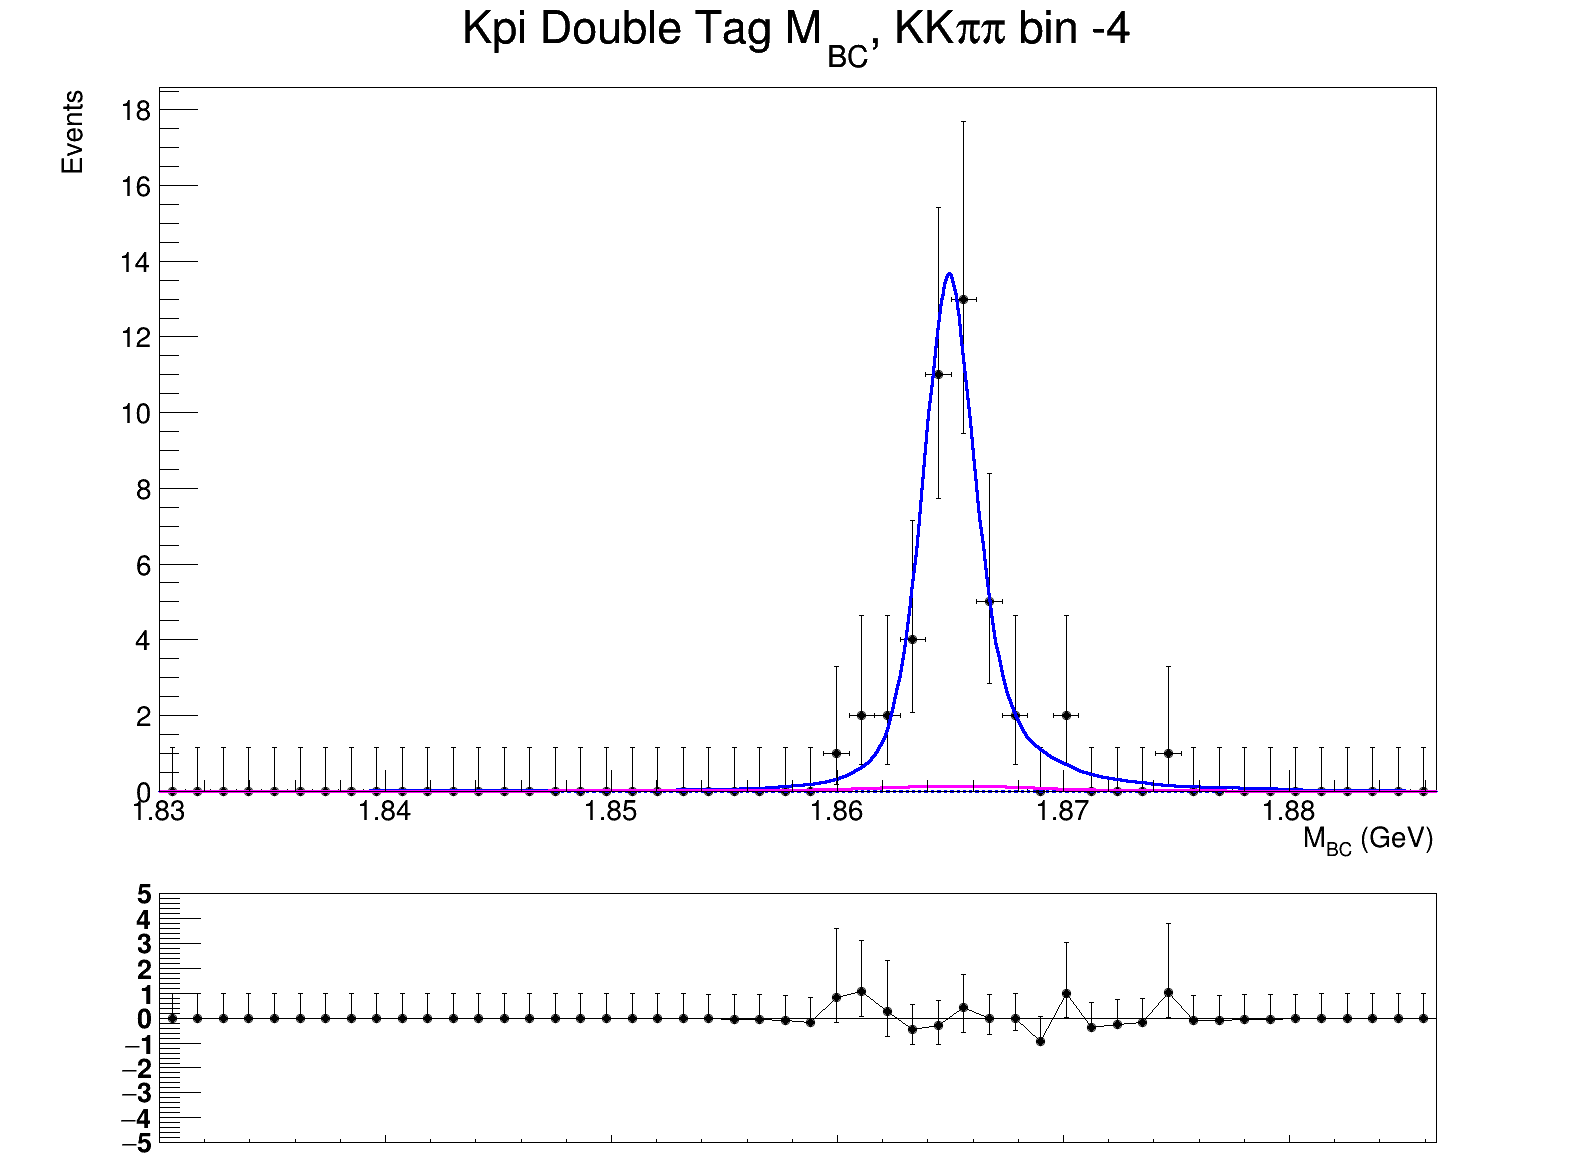
\includegraphics[width = 1.0\textwidth]{Plots/DoubleTagYield_DoubleTag_Flavour_KKpipi_vs_Kpi_SignalBinM4_TagBin0.png}
      \caption{$K\pi$}
    \end{subfigure}
    \begin{subfigure}{0.35\textwidth}
      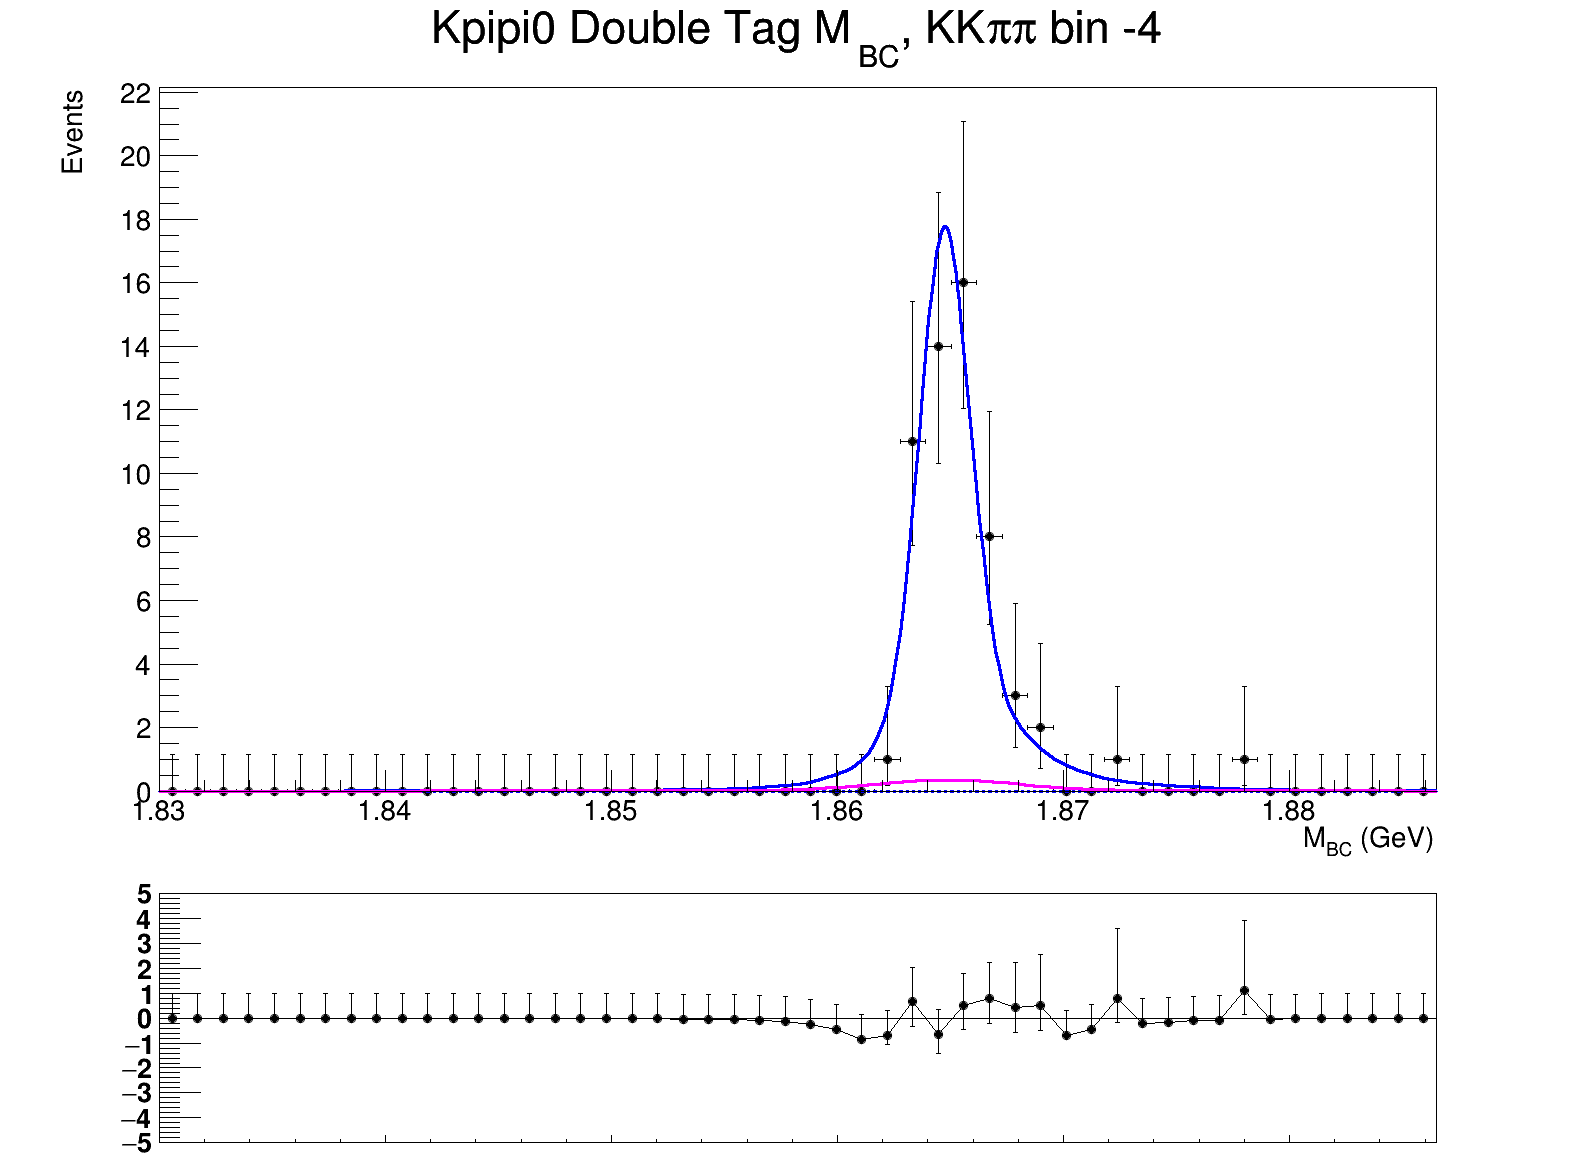
\includegraphics[width = 1.0\textwidth]{Plots/DoubleTagYield_DoubleTag_Flavour_KKpipi_vs_Kpipi0_SignalBinM4_TagBin0.png}
      \caption{$K\pi\pi^0$}
    \end{subfigure}%
    \begin{subfigure}{0.35\textwidth}
      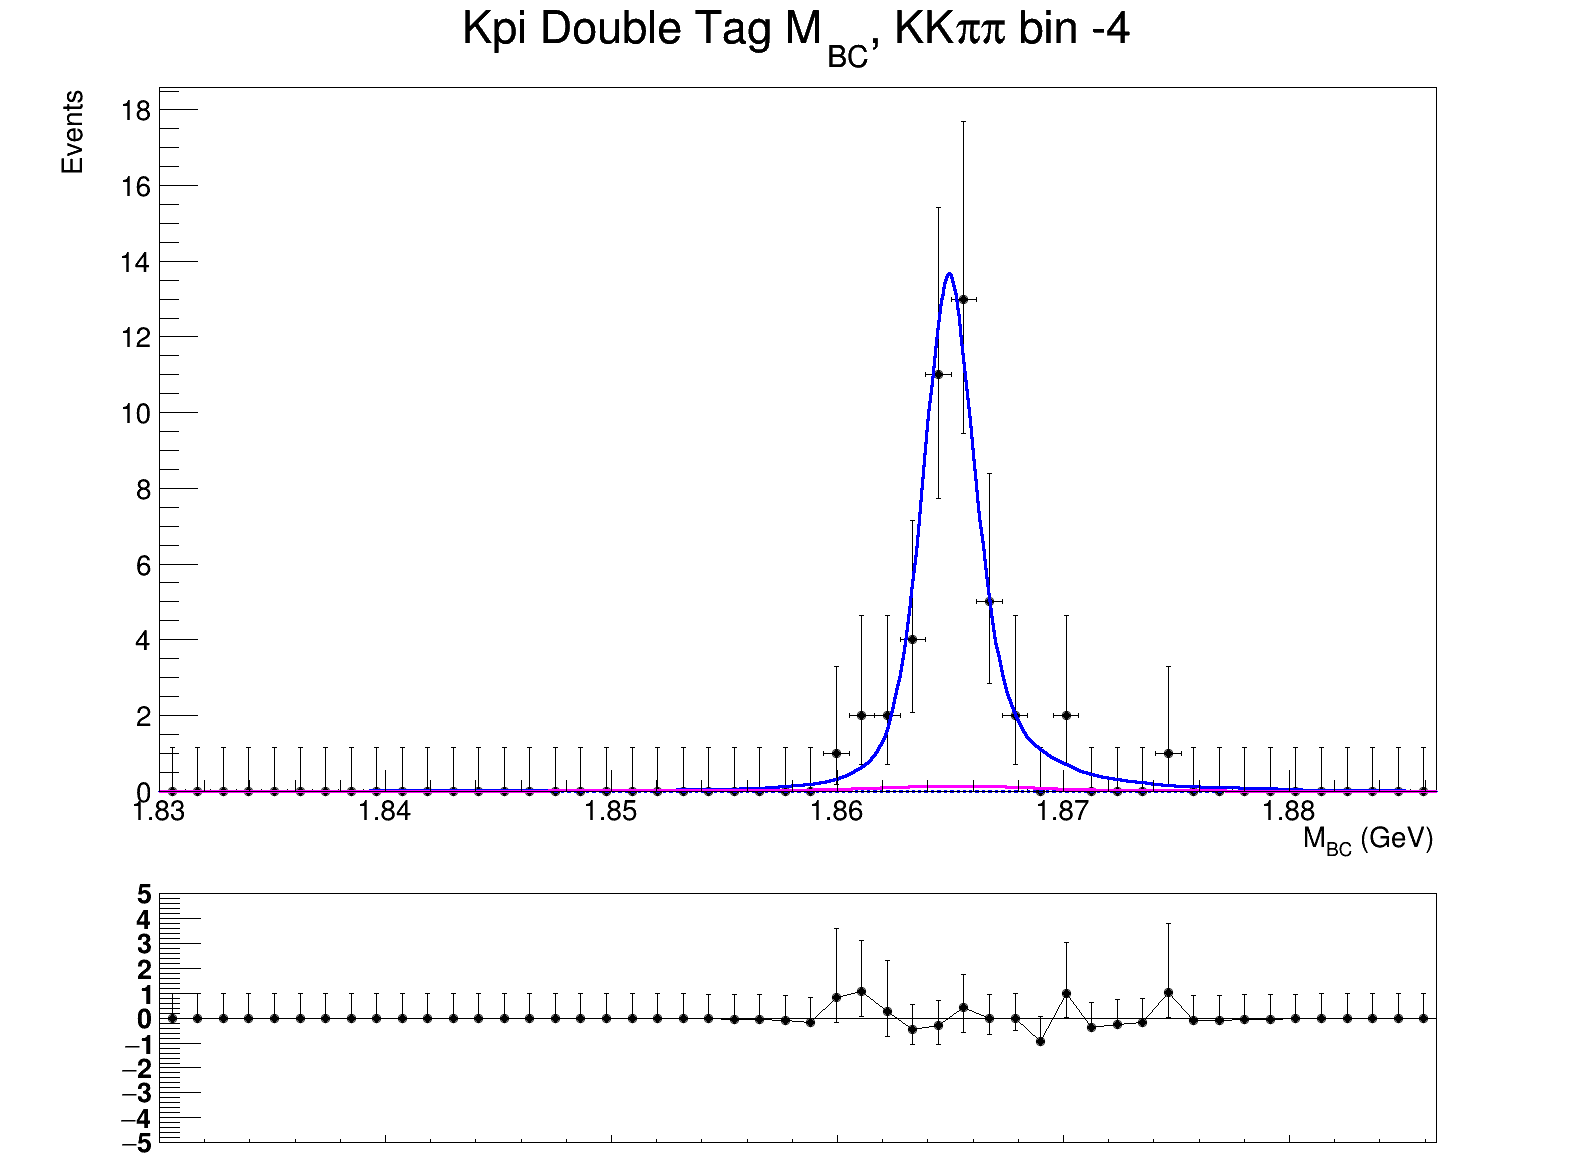
\includegraphics[width = 1.0\textwidth]{Plots/DoubleTagYield_DoubleTag_Flavour_KKpipi_vs_Kpi_SignalBinM4_TagBin0.png}
      \caption{$K\pi\pi\pi$}
    \end{subfigure}
  \end{figure}
\end{frame}

\begin{frame}{Measurement of fractional bin yields $K_i$}
  \begin{figure}
    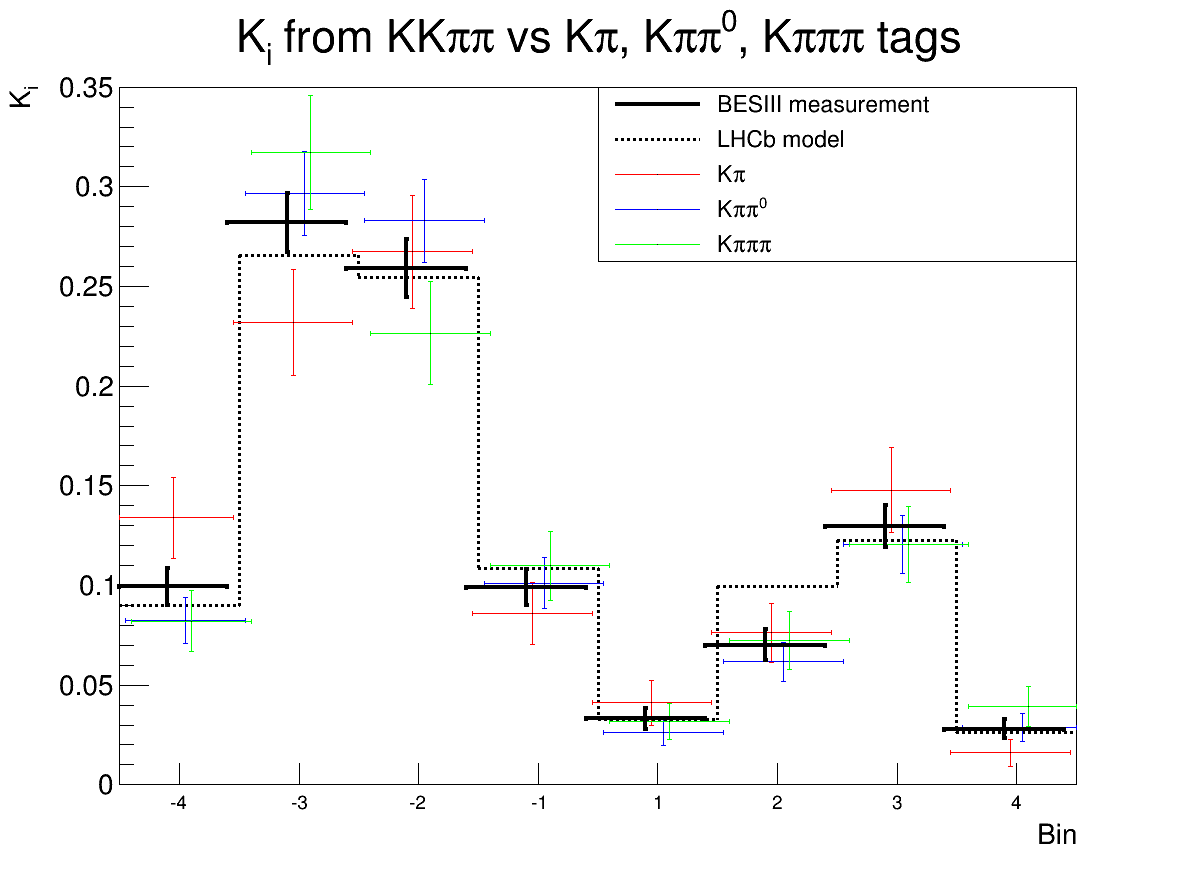
\includegraphics[width = 0.80\textwidth]{Plots/Ki_Measured_vs_Model.png}
  \end{figure}
  \vspace{-0.6cm}
  \begin{center}
    \Large Model agrees well with data so far!
  \end{center}
\end{frame}

\subsection{Measurement of CP-even fraction \texorpdfstring{$F_+$}{F+}}

\begin{frame}{Measurement of CP-even fraction $F_+$}
  \begin{itemize}
    \setlength\itemsep{1.0em}
    \item{CP tag yields too small for strong-phase analysis...}
    \item{Measure CP-even fraction $F_+$ instead}
    \begin{itemize}
      \setlength\itemsep{1.0em}
      \item{$F_+ = 1$ for CP even tags, $F_+ = 0$ for CP odd tags}
      \item{$2F_+ - 1$ is the average cosine of the strong-phase}
    \end{itemize}
    \item{$F_+$ is an input to GLW analyses of $\gamma$}
    \item{Good cross check of data-model agreement}
    \item{$KK\pi\pi$ model prediction: $F_+ = 0.74$ ($2F_+ - 1 = 0.47$)}
  \end{itemize}
\end{frame}

\begin{frame}{Measurement of CP-even fraction $F_+$}
  Strategy for measuring $F_+$:
  \begin{itemize}
    \setlength\itemsep{0.5em}
    \item{Measure double tag yield of CP tags \textit{without} binning}
    \item{Normalize double tag yields with single tag yields}
    \item{$\frac{N^{\rm DT}}{N^{\rm ST}} = \rm{BF}(D^0\to KK\pi\pi)\times\big(1\pm(2F_+ - 1)\big)$}
  \end{itemize}
  \begin{figure}
    \centering
    \vspace{-0.2cm}
    \begin{subfigure}{0.45\textwidth}
      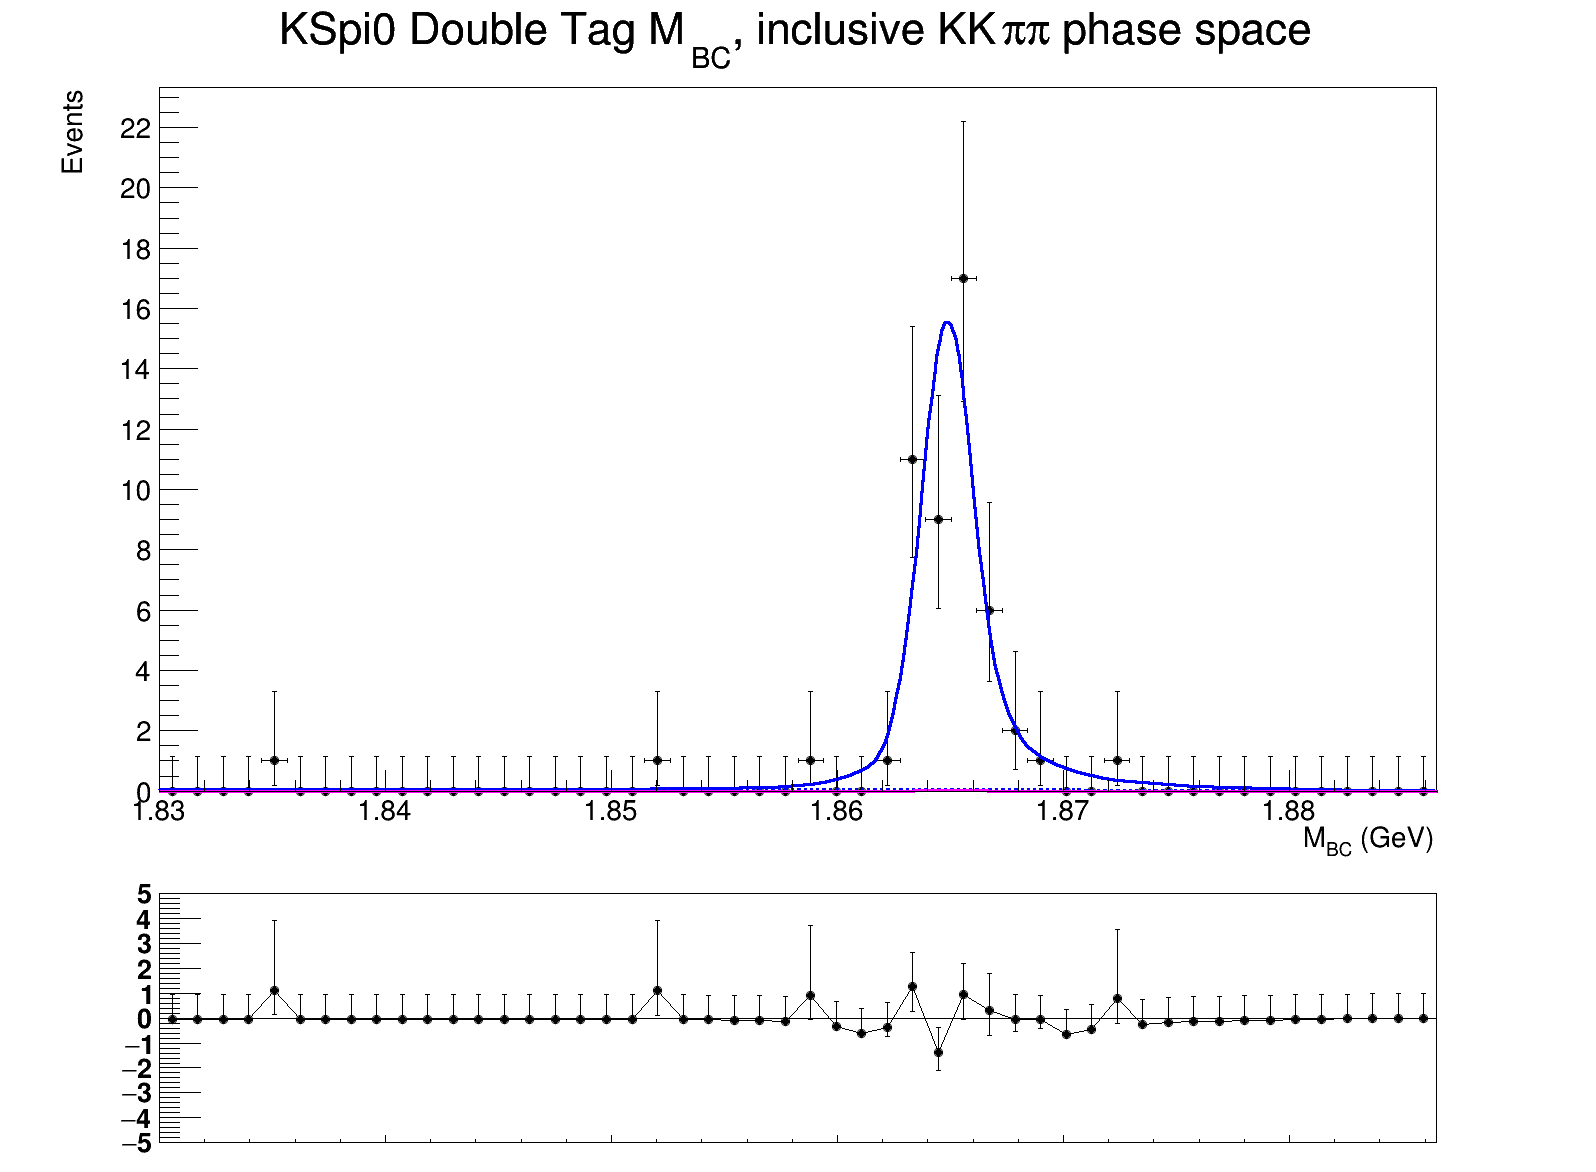
\includegraphics[width = 1.0\textwidth]{Plots/DoubleTagYield_DoubleTag_CP_KKpipi_vs_KSpi0_SignalBin0.png}
      \caption{$K_S\pi^0$}
    \end{subfigure}%
    \begin{subfigure}{0.45\textwidth}
      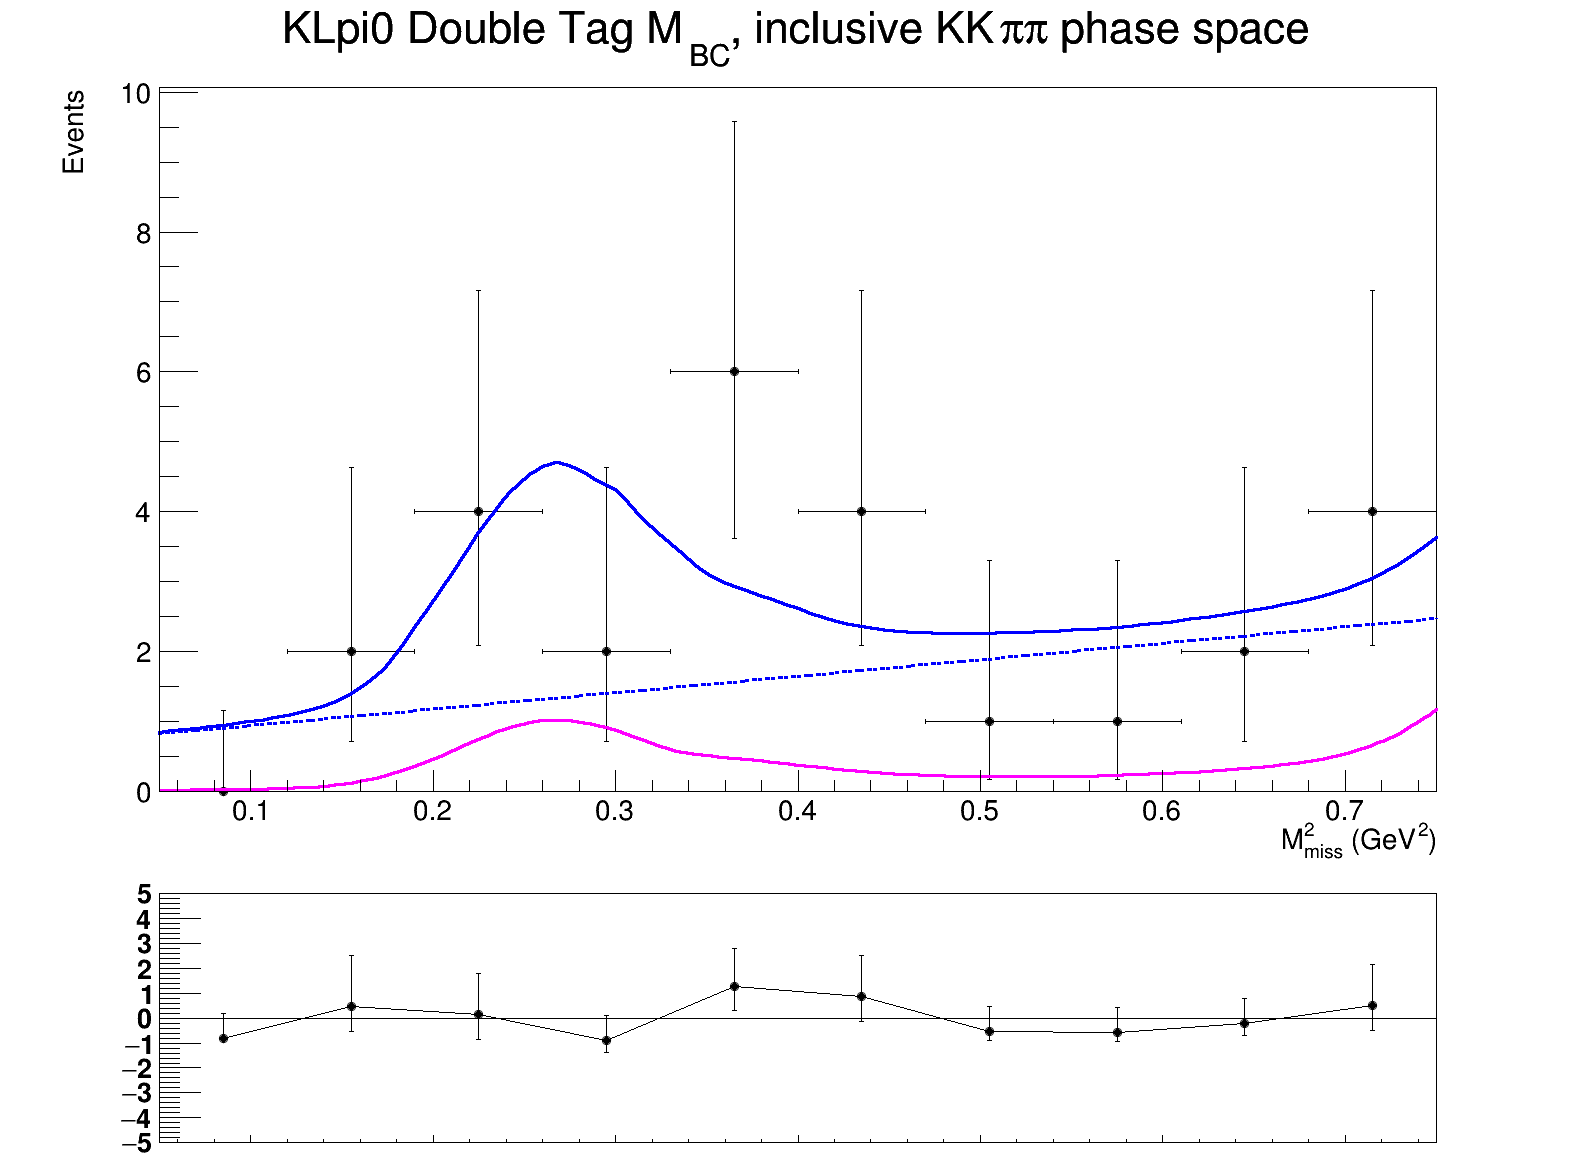
\includegraphics[width = 1.0\textwidth]{Plots/DoubleTagYield_DoubleTag_CP_KKpipi_vs_KLpi0_SignalBin0.png}
      \caption{$K_L\pi^0$}
    \end{subfigure}
  \end{figure}
\end{frame}

\begin{frame}{Measurement of CP-even fraction $F_+$}
  \begin{figure}
    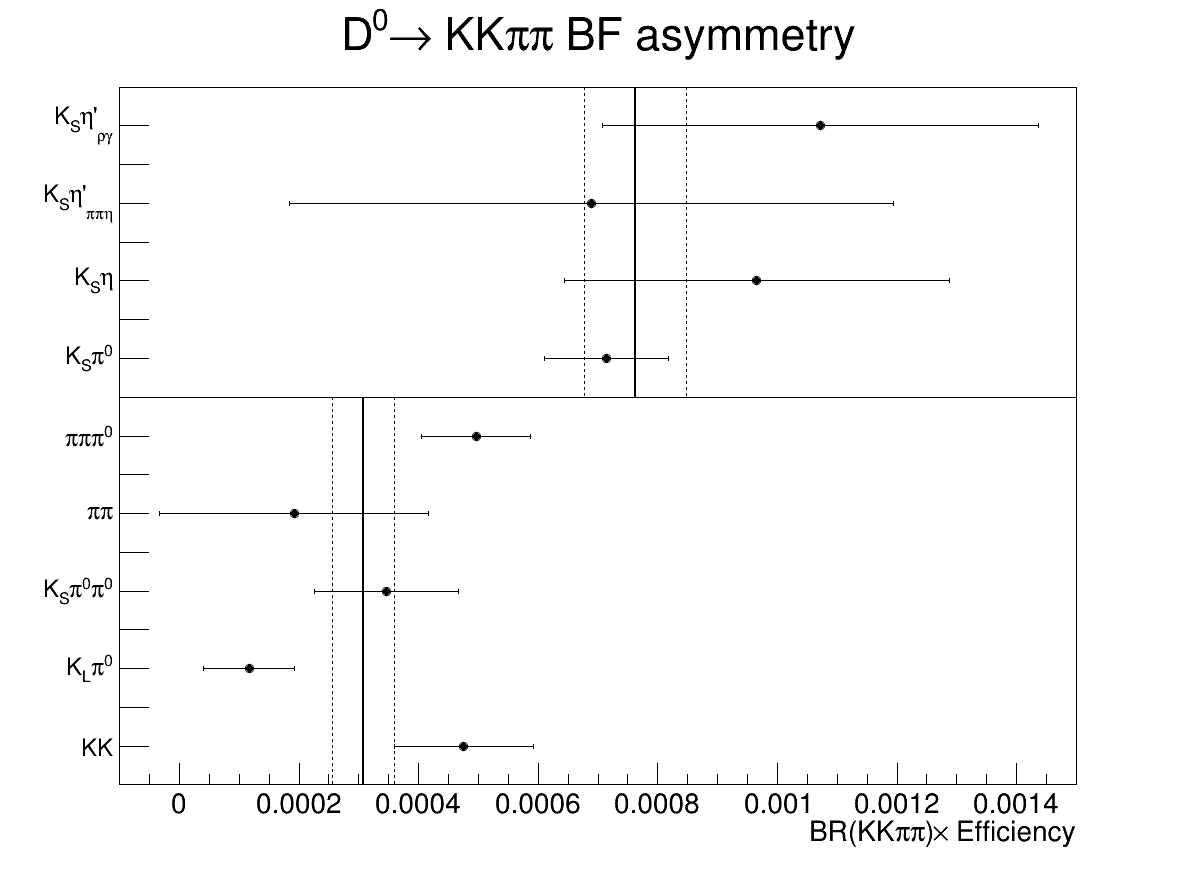
\includegraphics[width = 0.80\textwidth]{Plots/CPeven_fraction_combination.png}
  \end{figure}
  \vspace{-0.6cm}
  \begin{center}
    \large Fit result: $F_+ = \SI{0.71(4)}{}$ \\
    \large Model prediction: $F_+ = 0.74$
  \end{center}
\end{frame}

\section{Summary}

\begin{frame}{Summary}
  \begin{itemize}
    \setlength\itemsep{1.5em}
    \item{LHCb:}
    \begin{itemize}
      \setlength\itemsep{1.5em}
      \item{$B^\pm\to(K^+K^-\pi^+\pi^-)_Dh^\pm$ analysis in B2OC WG review}
      \item{Very encouraging feedback so far}
    \end{itemize}
    \item{BESIII:}
    \begin{itemize}
      \setlength\itemsep{1.5em}
      \item{Fractional bin yields $K_i$ agree well with model}
      \item{CP-even fraction $F_+$ shows good agreement with model, but low yields}
      \item{Will include $K_{S, L}\pi\pi$ tags}
    \end{itemize}
  \end{itemize}
  \begin{center}
    \huge Thank you!
  \end{center}
\end{frame}

\end{document}
